\chapter{航天器姿态运动学}
\thispagestyle{empty}

\section{航天器常用坐标系}
\subsection{基本概念}
\vspace*{-1em}

\defination[天体坐标系基本概念]
{
	\dy[天球]{{\text{T}}Q}\quad 指一个以地球质心$M$为中心,半径$r$为任意长的一个假想的球体 。其目的是将天体沿观测者视线投影到球面上,以便于研究天体及其相互关系。\\
	\hspace*{2.2em}\dy[黄道平面]{HDPM}\quad 由于地球绕太阳公公转而产生的,即地球公转轨道在天球上的反映称为黄道。它和赤道面相交于春分点和秋分点。\\
	\hspace*{2.2em}\dy[春分点]{CFD}\quad 指太阳从难向北在黄赤道上的交点。
}

\begin{figure}[!htb]
	\begin{minipage}{0.45\linewidth}
		\centering
		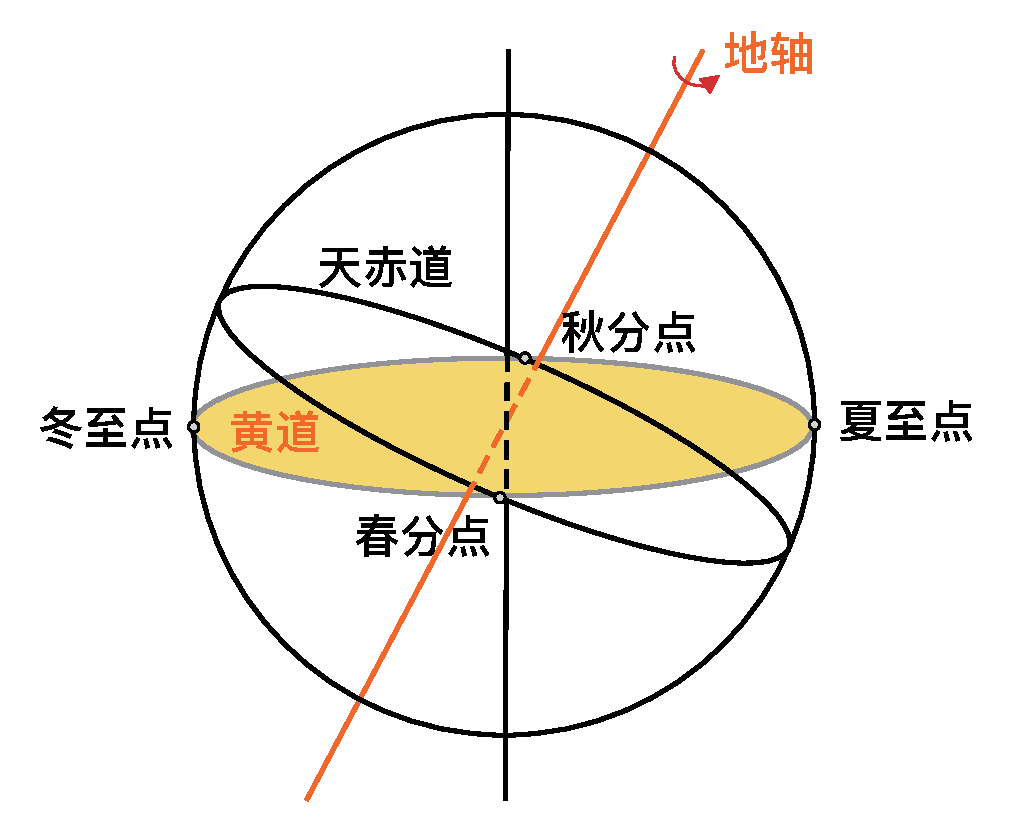
\includegraphics[width=\linewidth]{pic/基本概念}
		\caption{天球坐标系的基本概念}
		\label{基本概念}
	\end{minipage}
	\begin{minipage}{0.55\linewidth}
		\centering
		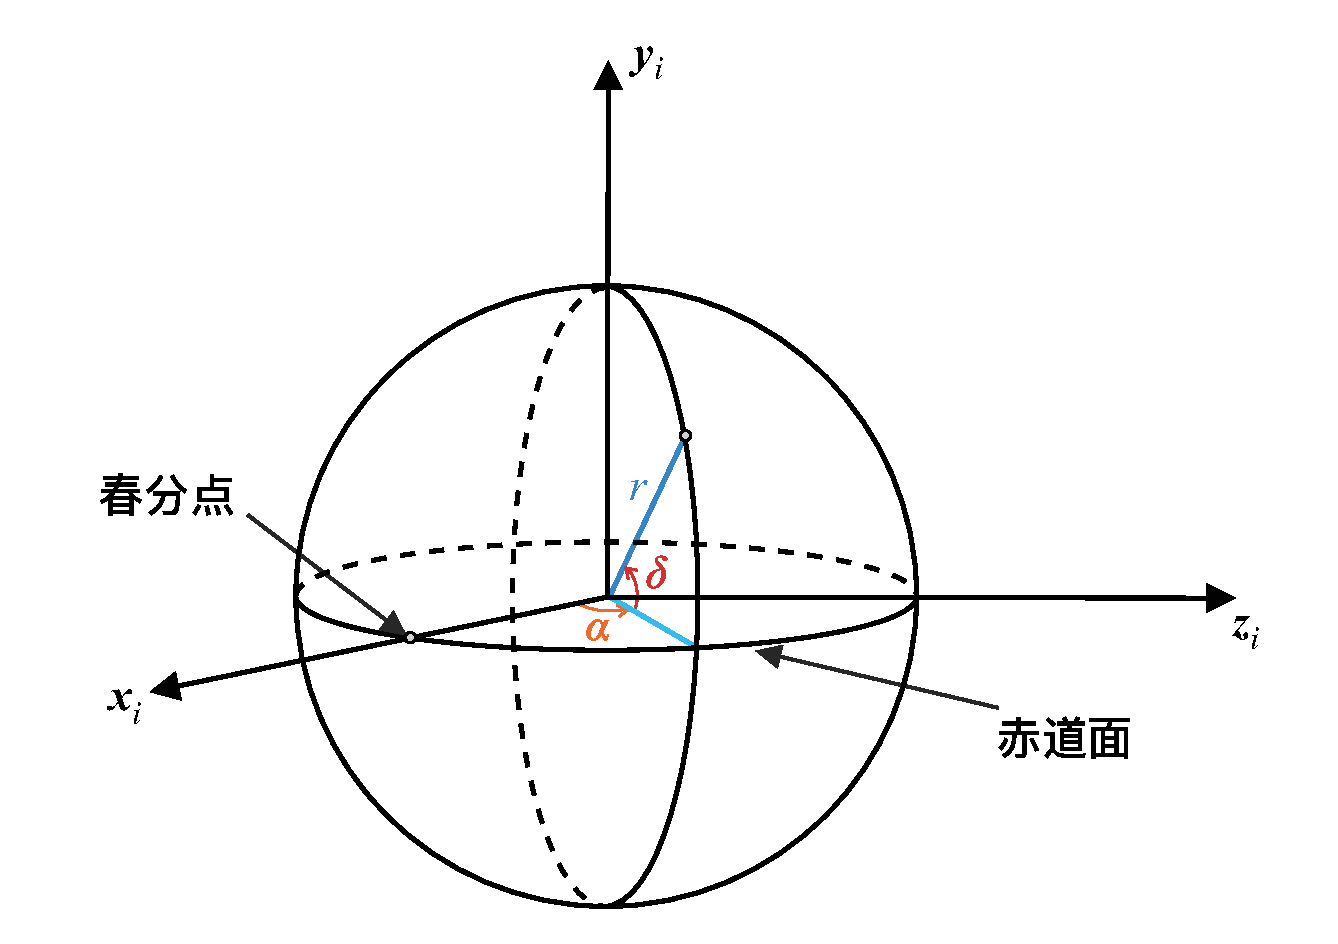
\includegraphics[width=\linewidth]{pic/地惯}
		\vspace*{-2.9em}
		\caption{地心赤道惯性坐标系}
		\label{地惯}
	\end{minipage}
\end{figure}


\subsection{地心赤道惯性坐标系}
\vspace*{-1em}

\defination[地心赤道惯性坐标系]
{
	如图 \ref{地惯} 所示,\dy[地心第一赤道坐标系]{DXDYCDZBX},简称为\dy[惯性坐标系]{GXZBX}。$X$轴在地球赤道平面内,指向赤道平面与黄道平面的相交线交点(春分点)。$Z$轴垂直于赤道平面,与地球自转角速度矢量方向一致。J2000的地心平赤道、平春分点的地心赤道坐标系。
}


\subsection{地心赤道旋转坐标系}
\vspace*{-1em}

\defination[地心赤道坐标系]
{
	如图 \ref{地心旋转} 所示,\dy[地心赤道旋转坐标系]{DXCDXZZBX},也叫\dy[地心第四赤道坐标系]{DXDSCDZBX}。$X$轴在赤道平面内,指向\dy[格林威治子午线]{GLNZZWX},$Z$轴垂直于赤道平面,与地球自转角速度矢量方向一致。$\lambda$是地理经度,从格林威治子午线向东度量,$\phi$是地心纬度。
}

\begin{figure}[!htb]
	\begin{minipage}{0.485\linewidth}
		\centering
		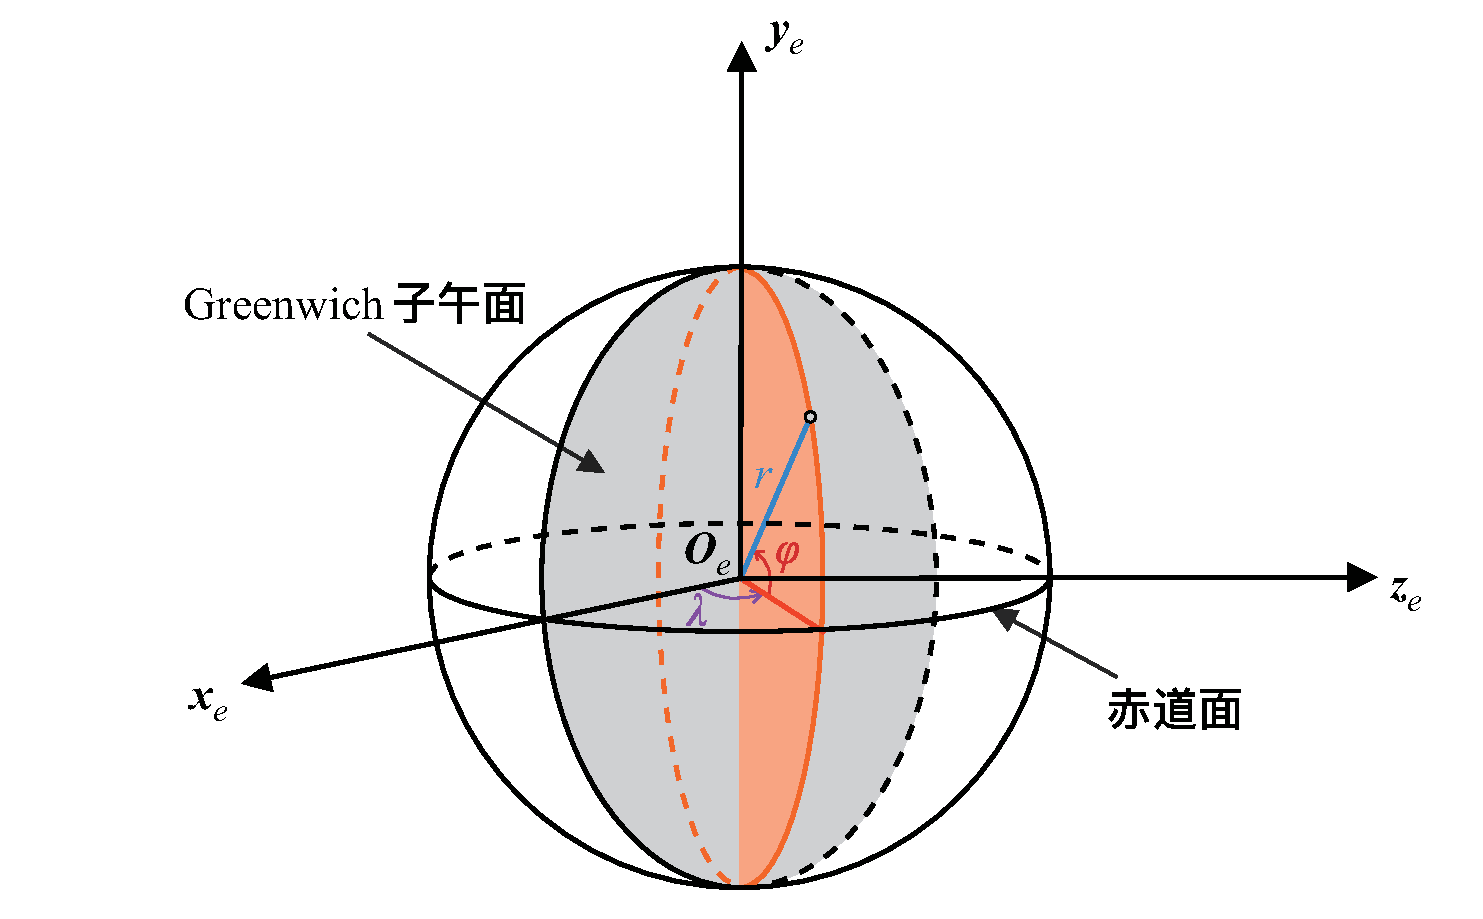
\includegraphics[width=\linewidth]{pic/地心旋转}
		\caption{地心赤道旋转坐标系}
		\label{地心旋转}
	\end{minipage}
	\begin{minipage}{0.515\linewidth}
		\centering
		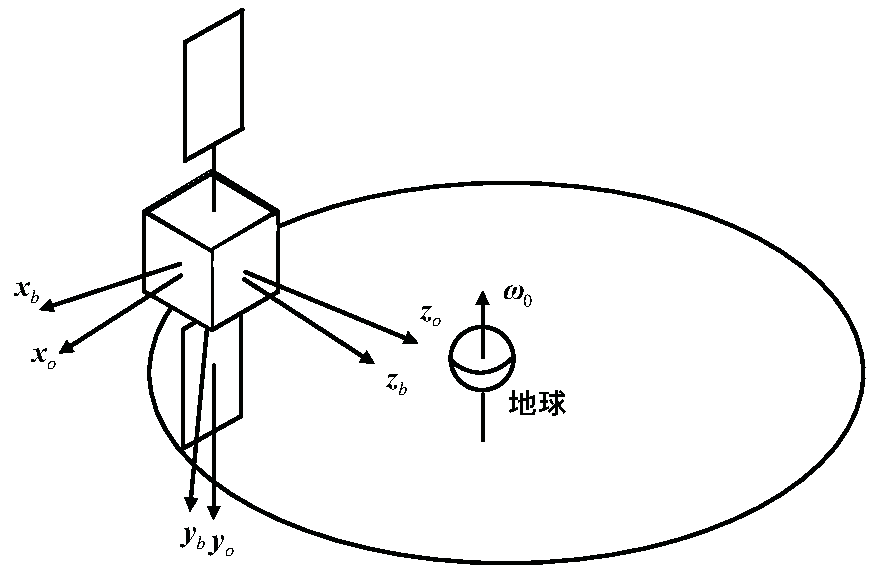
\includegraphics[width=\linewidth]{pic/轨道星体}
		\caption{轨道坐标系和星体坐标系}
		\label{轨道星体}
	\end{minipage}
\end{figure}


\subsection{轨道坐标系和星体坐标系}
\vspace*{-1em}

\defination[地心赤道坐标系]
{
	\dy[轨道坐标系]{DY}\quad 原点在飞行器质心,$z_o$轴指向地心,$x_o$轴在轨道面内与$z_o$轴垂直,指向速度方向,$y_o$轴在轨道平面法线方向,与$x_o$,$z_o$轴成右手正交坐标系。\\
	\hspace*{2.2em}\dy[星体坐标系]{X{\text{T}}ZBX}\quad 原点在质心,$x_b$轴为\dy[滚动轴]{GDZ},$y_b$轴为\dy[俯仰轴]{FYZ},$z_b$轴为\dy[偏航轴]{PHZ}。(对地定向航天器)
}


\section{姿态参数}
\subsection{方向余弦矩阵}
	对于坐标系原点重合的两个不同的坐标系$S_a$和$S_b$,坐标基分别为$\bm{e}_a$和$\bm{e}$
,对于矢量$\bm{u}$在两个坐标系下的分解,有
\begin{equation}
	\bm{u} = \bm{e}_b^{\text{T}}u_b = \bm{e}_a^{\text{T}}u_a
\end{equation}
两边同时乘以$\bm{e}_b$,得
\begin{equation*}
	\bm{e}_b \bm{e}_b^{\text{T}} u_b = \bm{e}_b \bm{e}_a^{\text{T}} u_a \quad \Rightarrow \quad u_b = \bm{e}_b\bm{e}_au_a^{\text{T}}
\end{equation*}
为此我们定义坐标系$S_a$变换为坐标系$S_b$的\dy[方向余弦矩阵]{FXYXJZ}为
\begin{equation}
	\bm{C}_{ba} = \bm{e}_b \bm{e}_a^{\text{T}}
	=
	\begin{bmatrix}
		\bm{i}_b \cdot \bm{e}_a^{\text{T}} \\
		\bm{j}_b \cdot \bm{e}_a^{\text{T}} \\
		\bm{k}_b \cdot \bm{e}_a^{\text{T}} 
	\end{bmatrix}
	=
	\begin{bmatrix}
		\bm{i}_b \cdot \bm{i}_a & \bm{i}_b \cdot \bm{j}_a & \bm{i}_b \cdot \bm{k}_a \\
		\bm{j}_b \cdot  \bm{i}_a & \bm{j}_b \cdot \bm{j}_a & \bm{j}_b \cdot \bm{k}_a \\
		\bm{k}_b \cdot  \bm{i}_a & \bm{k}_b \cdot \bm{j}_a & \bm{k}_b \cdot \bm{k}_a 
	\end{bmatrix}
	=
	\begin{bmatrix}
		C_{11} & C_{12} & C_{13} \\
		C_{21} & C_{22} & C_{23} \\
		C_{31} & C_{32} & C_{33}
	\end{bmatrix}
\end{equation}
方向余弦矩阵有以下几个特征:

\newpage

\sssection[6个约束方程]
\noa[1] 模值约束
\begin{equation}
	\begin{cases}
		\,\big|\bm{i}_b\big|^2 = C_{11}^2 + C_{12}^2 + C_{13}^2 = 1\\
		\,\big|\bm{j}_b\big|^2 = C_{21}^2 + C_{22}^2 + C_{23}^2 = 1\\
		\,\big|\bm{k}_b\big|^2 = C_{31}^2 + C_{32}^2 + C_{33}^2 = 1
	\end{cases}
\end{equation}
\proof 由于$\bm{i}_b, \bm{j}_b, \bm{k}_b$的模值为1(空间绝对),所以将它们投影到坐标系$S_a$后模值仍然为1,即
\begin{equation*}
	\begin{cases}
		\,\big|\bm{i}_b \cdot \bm{e}_a^{\text{T}}\big|^2 = \big|\bm{i}_b\big|^2 = 1\\
		\,\big|\bm{j}_b \cdot \bm{e}_a^{\text{T}}\big|^2 = \big|\bm{j}_b\big|^2 = 1\\
		\,\big|\bm{k}_b \cdot \bm{e}_a^{\text{T}}\big|^2 = \big|\bm{k}_b\big|^2 = 1\\
	\end{cases}
	\qquad \Longrightarrow \qquad 
	\begin{cases}
		\,\big|\bm{i}_b\big|^2 = C_{11}^2 + C_{12}^2 + C_{13}^2 = 1\\
		\,\big|\bm{j}_b\big|^2 = C_{21}^2 + C_{22}^2 + C_{23}^2 = 1\\
		\,\big|\bm{k}_b\big|^2 = C_{31}^2 + C_{32}^2 + C_{33}^2 = 1
	\end{cases}
\end{equation*}

\noa[2] 几何约束
\begin{equation}
	\begin{cases}
		\,\bm{i}_b \cdot \bm{j}_b = C_{11}C_{21} + C_{12}C_{22} + C_{13}C_{23} = 0 \\
		\,\bm{i}_b \cdot \bm{k}_b = C_{11}C_{31} + C_{12}C_{32} + C_{13}C_{33} = 0 \\
		\,\bm{j}_b \cdot \bm{k}_b = C_{21}C_{31} + C_{22}C_{32} + C_{23}C_{33} = 0
	\end{cases}
\end{equation}
\proof 由于$\bm{i}_b, \bm{j}_b, \bm{k}_b$两两正交(空间绝对),所以将它们投影到坐标系$S_a$后仍然满足几何关系,即
\begin{equation*}
	\begin{cases}
		\,\bm{i}_b \cdot \bm{j}_b = \big(\bm{i}_b \cdot \bm{e}_a^{\text{T}}\big) \cdot  \big(\bm{j}_b \cdot \bm{e}_a^{\text{T}}\big) = 0\\
		\,\bm{i}_b \cdot \bm{k}_b = \big(\bm{i}_b \cdot \bm{e}_a^{\text{T}}\big) \cdot \big(\bm{k}_b \cdot \bm{e}_a^{\text{T}}\big) = 0\\
		\,\bm{j}_b \cdot \bm{k}_b =\big(\bm{j}_b \cdot \bm{e}_a^{\text{T}}\big) \cdot \big(\bm{k}_b \cdot \bm{e}_a^{\text{T}}\big) = 0
	\end{cases}
	\qquad \Longrightarrow \qquad 
	\begin{cases}
		\,\bm{i}_b \cdot \bm{j}_b = C_{11}C_{21} + C_{12}C_{22} + C_{13}C_{23} = 0 \\
		\,\bm{i}_b \cdot \bm{k}_b = C_{11}C_{31} + C_{12}C_{32} + C_{13}C_{33} = 0 \\
		\,\bm{j}_b \cdot \bm{k}_b = C_{21}C_{31} + C_{22}C_{32} + C_{23}C_{33} = 0
	\end{cases}
\end{equation*}


\vspace*{0.5em}
\sssection[坐标变换矩阵是正交矩阵]

由于
\begin{equation*}
	\begin{cases}
		\,\bm{e}_b \cdot \bm{e}_b^{\text{T}} = \bm{e}_a \cdot \bm{e}_a^{\text{T}} = \bm{E}_3\\
		\,\bm{e}_b \cdot \bm{e}_b^{\text{T}} = \bm{C}_{ba}\bm{e}_a \cdot \big( \bm{C}_{ba} \bm{e}_a \big)^{\text{T}} =  \bm{C}_{ba}\bm{e}_a \cdot \bm{e}_a^{\text{T}} \bm{C}_{ba}^{\text{T}} 
	\end{cases}
	\quad \Rightarrow \quad \bm{E}_3 = \bm{C}_{ba} \cdot \big( \bm{e}_a \cdot \bm{e}_a^{\text{T}} \big) \cdot \bm{C}_{ba}^{\text{T}} =  \bm{C}_{ba} \cdot \bm{C}_{ba}^{\text{T}}
\end{equation*}
所以可以得到
\begin{equation}
	\bm{C}_{ba}^{\text{T}} = \bm{C}_{ba}^{-1}
\end{equation}
且有
\begin{equation}
	\bm{C}_{ab} = \bm{e}_a \cdot \bm{e}_b^{\text{T}} = \bm{e}_a \cdot \bm{e}_a^{\text{T}} \bm{C}_{ba}^{\text{T}} = \bm{C}_{ba}^{-1}
\end{equation}


\vspace*{0.5em}
\sssection[坐标变换矩阵的行列式为1]

由于矩阵乘积的行列式等于行列式的乘积且矩阵的转置的行列式等于矩阵的行列式,所以
\begin{equation}
	\det \big(\bm{C}_{ba}\big) \det \big(\bm{C}_{ba}^{\text{T}}\big) 
	= \big[ \det \big(\bm{C}_{ba} \big) \big]^2 
	= \det \big( \bm{C}_{ba} \cdot \bm{C}_{ba}^{\text{T}} \big) 
	= 1
	\quad \Rightarrow \quad 
	\det \big(\bm{C}_{ba}\big) = \pm 1
\end{equation}
而因为
\begin{equation*}
	\bm{C}_{ba}^{\text{T}} = \text{adj}\big( \bm{C}_{ba} \big) 
	\quad  \Rightarrow \quad 
	\bm{C}_{ba}^{-1} 
	= \dfrac{\text{adj}\big( \bm{C}_{ba} \big)}{\det \big( \bm{C}_{ba} \big)} 
	= \dfrac{\bm{C}_{ba}^{\text{T}}}{\det \big( \bm{C}_{ba} \big)} 
	= \dfrac{\bm{C}_{ba}^{-1}}{\det \big( \bm{C}_{ba} \big)}
\end{equation*}
因此
\begin{equation}
	\det \big( \bm{C}_{ba} \big) = + 1
\end{equation}

\clearpage


\sssection[相继运动的坐标变换矩阵]

对于坐标系原点重合的三个不同的坐标系$S_a$,$S_b$和$S_c$,有
\begin{equation*}
	\begin{cases}
		\, \bm{e}_b \cdot \bm{e}_a^{\text{T}} = \bm{C}_{ba} \\
		\, \bm{e}_c \cdot \bm{e}_b^{\text{T}} = \bm{C}_{cb} \\
		\, \bm{e}_c \cdot \bm{e}_a^{\text{T}} = \bm{C}_{ca}
	\end{cases}
	\quad \Rightarrow \quad 
	\bm{e}_c = \bm{C}_{ca} \bm{e}_a = \bm{C}_{cb}\bm{e}_b = \bm{C}_{cb} \bm{C}_{ba} \bm{e}_{a}
\end{equation*}
因此
\begin{equation}
	\bm{C}_{ca} = \bm{C}_{cb} \bm{C}_{ba}
\end{equation}
\vspace*{0.5em}


\subsection{欧拉角}
\vspace*{-1em}

\defination[基元旋转矩阵]
{
	\dy[基元旋转矩阵]{JYXZJZ}\quad 任何一个坐标变换可以看成是绕三个基本轴的旋转,这三个基本轴的坐标转换矩阵为基元旋转矩阵,如图 \ref{x}, \ref{y}, \ref{z} 所示,绕各个轴旋转的角度称为\dy[欧拉角]{OLJ}。每个坐标轴对应的基元旋转矩阵为
	\begin{equation}
		\bm{C}_x (\varphi) =
		\begin{bmatrix}
			1 & 0 & 0 \\
			0 & \cos \varphi & \sin \varphi \\
			0 & - \sin \varphi & \cos \varphi 
		\end{bmatrix}
		\qquad \quad
		\bm{C}_y (\theta) = 
		\begin{bmatrix}
			\cos \theta & 0 & - \sin \theta \\
			0 & 1 & 0 \\
			\sin \theta & 0 & \sin \theta 
		\end{bmatrix}
		\qquad \quad
		\bm{C}_z (\psi) = 
		\begin{bmatrix}
			\cos \psi & \sin \psi & 0 \\
			- \sin \psi &\cos \psi & 0 \\
			0 & 0 & 1
		\end{bmatrix}
	\end{equation}
	{	
		\centering
		\begin{minipage}{0.34\linewidth}
			\centering
			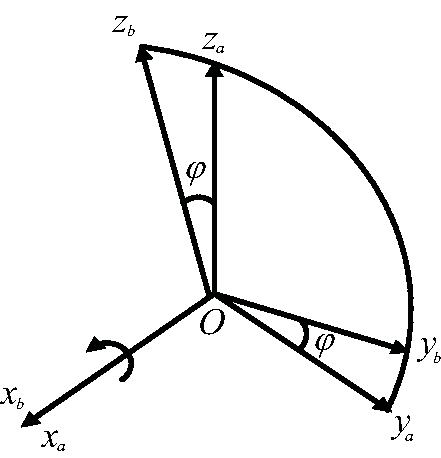
\includegraphics[width=0.77\linewidth]{pic/x}
			\vspace*{-0.5em}
			\captionof{figure}{绕$x$轴旋转}
			\label{x}
		\end{minipage}
		\begin{minipage}{0.3\linewidth}
			\centering
			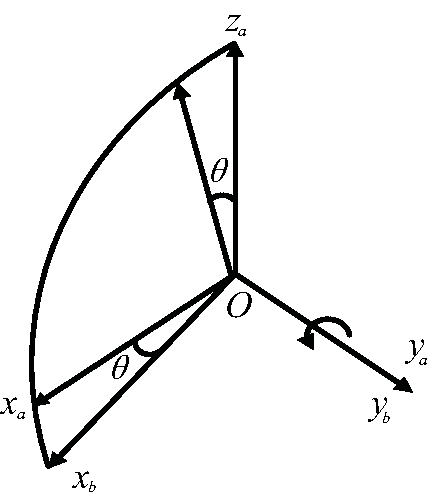
\includegraphics[width=0.78\linewidth]{pic/y}
			\vspace*{-0.5em}
			\captionof{figure}{绕$y$轴旋转}
			\label{y}
		\end{minipage}
		\begin{minipage}{0.34\linewidth}
			\centering
			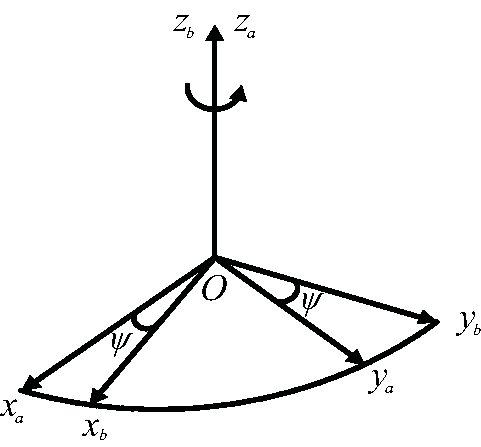
\includegraphics[width=0.85\linewidth]{pic/z}
			\vspace*{-0.5em}
			\captionof{figure}{绕$z$轴旋转}
			\label{z}
		\end{minipage}
	}
}

下面给出两种基元旋转矩阵表示的坐标变换。
\vspace*{0.5em}

\sssection[$ZXZ$旋转顺序]

如图 \ref{ZXZ} 所示,方向余弦矩阵和$ZXZ$顺序欧拉角的关系为
\begin{equation}
	\bm{C}_{ba} = \bm{C}_z(\varphi) \bm{C}_x(\theta) \bm{C}_z(\psi) = 
	\begin{bmatrix}
		\cos \varphi \cos \psi - \sin \varphi \cos \theta \sin \psi & \cos \varpi \sin \psi + \sin \varphi \cos \theta \cos \psi & \sin \varphi \sin \theta \\
		- \sin \varphi \cos \psi - \cos \varphi \cos \theta \sin \psi & -\sin \varphi \sin \psi + \cos \varphi \cos \theta \cos \psi & \cos \varphi \sin \theta \\
		\sin \theta \sin \psi & -\sin \theta \cos \psi & \cos \theta 
	\end{bmatrix}
\end{equation}
通过与方向余弦矩阵的对应项进行对比,可以计算得到
\begin{equation}
	\begin{cases}
		\, \psi = -\tan^{-1}\left( \dfrac{C_{31}}{C_{32}} \right) \\
		\, \theta = \cos^{-1}\big( C_{33} \big) \\
		\, \varphi = \tan^{-1} \left( \dfrac{C_{13}}{C_{23}} \right)
	\end{cases}
	\label{eq:zxz}
\end{equation}
\clearpage

\begin{figure}[!htb]
	\begin{minipage}{0.5\linewidth}
		\centering
		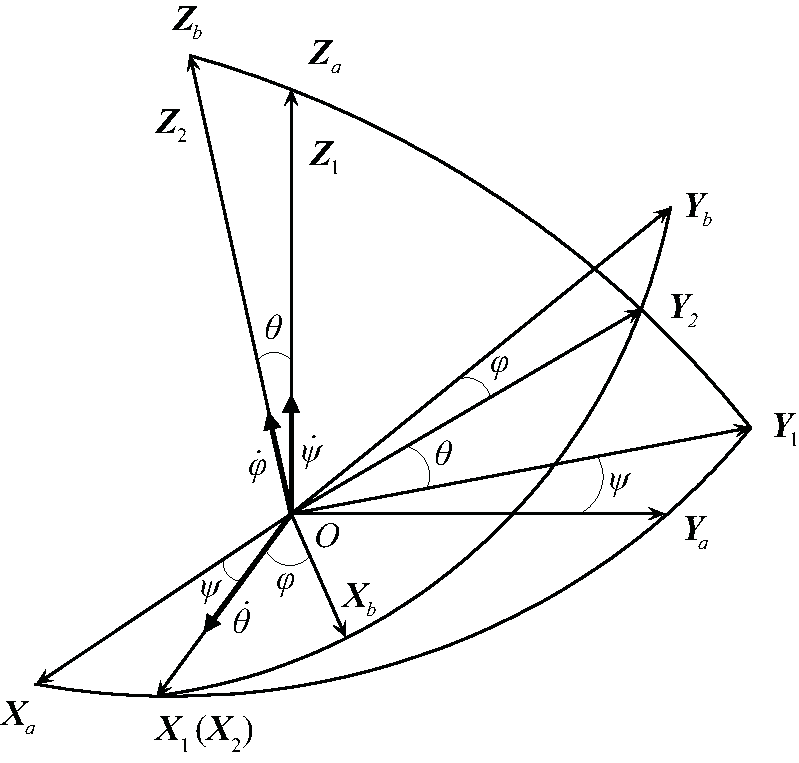
\includegraphics[width=0.8\linewidth]{pic/ZXZ}
		\caption{$ZXZ$顺序欧拉角旋转}
		\label{ZXZ}
	\end{minipage}
	\begin{minipage}{0.5\linewidth}
		\centering
		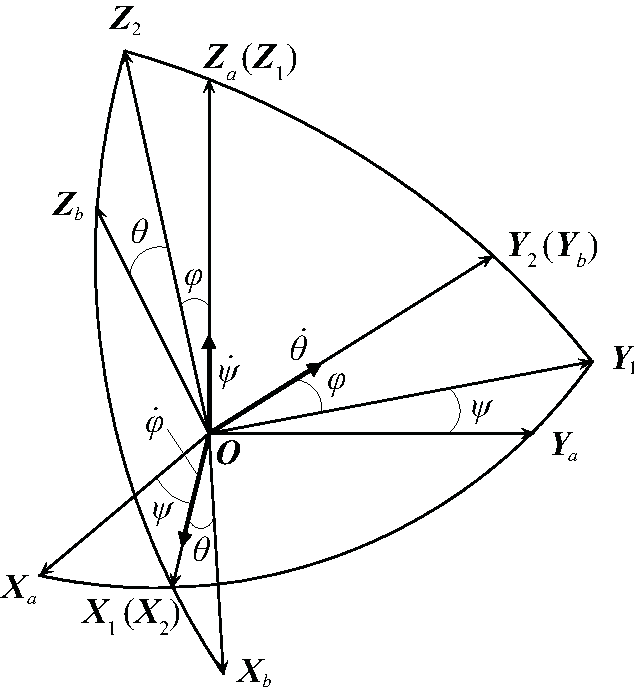
\includegraphics[width=0.695\linewidth]{pic/ZXY}
		\caption{$ZXY$顺序欧拉角旋转}
		\label{ZXY}
	\end{minipage}
\end{figure}
由公式 \eqref{eq:zxz} 可知,若欧拉角$\theta = 0\degree$,则欧拉转动处于奇异状态,欧拉角$\psi, \varphi$不能唯一确定。因此,$\theta$的取值范围为$0\degree<\theta<180\degree$。
\vspace*{1em}

\sssection[$ZXY$旋转顺序]

如图 \ref{ZXY} 所示,方向余弦矩阵和$ZXY$顺序欧拉角的关系
\begin{equation}
	\bm{C}_{ba} = \bm{C}_y(\theta)\bm{C}_x(\varphi)\bm{C_z(\psi)} =
	\begin{bmatrix}
		\cos \theta \cos \psi - \sin \varphi \sin \theta \sin \psi & \cos \theta \sin \psi + \sin \varphi \sin \theta \cos \psi & -\cos \varphi \sin \theta \\
		-\cos \varphi \sin \psi & \cos \varphi \cos \psi & \sin \varphi \\
		\sin \theta \cos \varphi + \sin \varphi \cos \theta \sin \psi & \sin \theta \sin \psi - \sin \varphi \cos \theta \cos \psi & \cos \varphi \cos \theta 
	\end{bmatrix}
\end{equation}
通过与方向余弦矩阵的对应项进行对比,可以计算得到
\begin{equation}
	\begin{cases}
		\, \psi = -\tan^{-1}\left( \dfrac{C_{21}}{C_{22}} \right) \\
		\, \theta = \sin^{-1}\big( C_{23} \big) \\
		\, \varphi = \tan^{-1} \left( \dfrac{C_{13}}{C_{33}} \right)
	\end{cases}
	\label{eq:zxy}
\end{equation}

由公式 \eqref{eq:zxy} 可知,若欧拉角$\theta = \pm 90 \degree$,则欧拉转动处于奇异状态,欧拉角$\psi, \varphi$在同一平面转动,不能唯一确定。
\vspace*{0.5em}



\subsection{欧拉轴角}
\label{sec: 欧拉轴角}
\vspace*{-1.5em}

\defination[欧拉轴 / 角]
{
	坐标系$S_b$相对坐标系$S_a$的姿态参数可以用单位矢量$\bm{e}$在参考坐标系$S_a$的三个分量$e_x, e_y, e_z$以及绕此转轴的转角$\varPhi$这4个参数来描述,称为\dy[欧拉轴 / 角]{OLZJ}参数。矢量$\bm{e}$称为\dy[欧拉轴]{OLZ},$\varPhi$称为\dy[欧拉转角]{OLZJ}。
}

\sssection[欧拉轴 / 角求方向余项矩阵]

方向余项矩阵$\bm{C}_{ba}$可由欧拉轴 / 角参数$\bm{e}, \varPhi$得到,即
\begin{align}
	\bm{C}_{ba} 
	& = \cos \varPhi \bm{E}_e + \big( 1 - \cos \varPhi \big) \bm{e} \bm{e}^{\text{T}} - \sin \varPhi \bm{e}^{\times} \notag \\
	& = 
	\begin{bmatrix}
		\cos \varPhi + e_x^2 \big( 1 - \cos \varPhi \big) & e_x e_y \big( 1 - \cos \varPhi \big) + e_z \sin \varPhi & e_x e_z \big( 1 - \cos \varPhi \big) - e_y \sin \varPhi \\
		e_x e_y \big( 1 - \cos \varPhi \big) - e_z \sin \varPhi & \cos \varPhi + e_y^2 \big( 1 - \cos \varPhi \big) & e_y e_z \big(1 - \cos \varPhi \big) + e_x \sin \varPhi \\
		e_x e_z \big( 1 - \cos \varPhi \big) + e_y \sin \varPhi & e_y e_z \big( 1- \cos \varPhi \big) - e_x \sin \varPhi & \cos \varPhi + e_z^2 \big( 1- \cos \varPhi \big)
	\end{bmatrix}
\end{align}
\clearpage
\vspace*{-3em}

\proof 如图 \ref{欧拉轴} 所示,设矢量$\bm{a}$是固定在坐标系$S_a$的任意矢量,矢量$\bm{b}$是固定于坐标系$S_b$中的矢量。将矢量$\bm{a}$绕轴$\bm{e}$旋转一个角度$\varPhi$后得到矢量$\bm{b}$。首先将矢量$\bm{a}$,矢量$\bm{b}$沿轴$\bm{e}$方向和垂直于轴$\bm{e}$方向分解,其平行分量$\bm{a}_{\parallel} = \bm{b}_{\parallel} = \bm{e}$相等,即旋转前后不变,可以发现旋转仅与垂直分量$\bm{a}_{\perp}, \bm{b}_{\perp}$有关。

\begin{figure}[!htb]
	\begin{minipage}{0.31\linewidth}
		\centering
		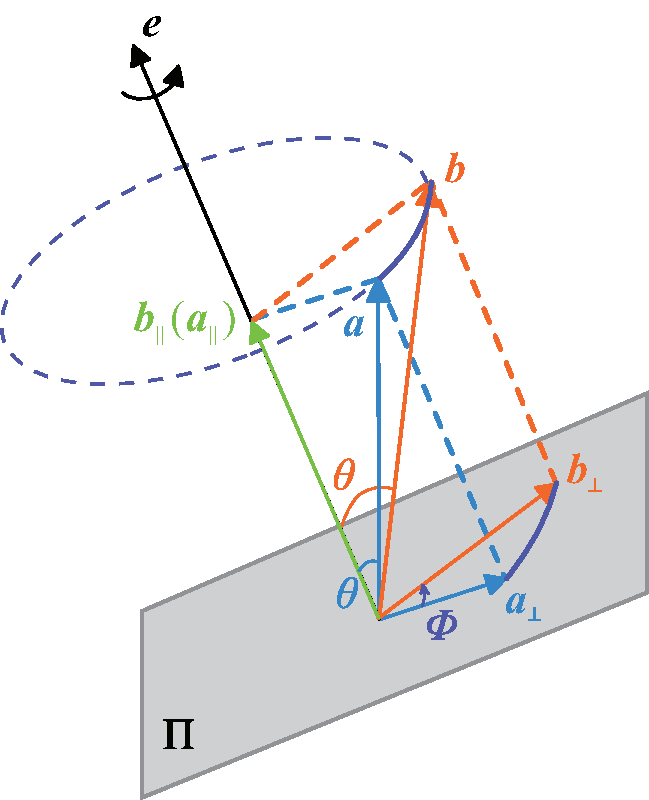
\includegraphics[width=0.9\linewidth]{pic/欧拉轴}
		\vspace*{-1.2em}
		\caption{欧拉轴旋转分解图}
		\label{欧拉轴}
	\end{minipage}
	\begin{minipage}{0.348\linewidth}
		\centering
		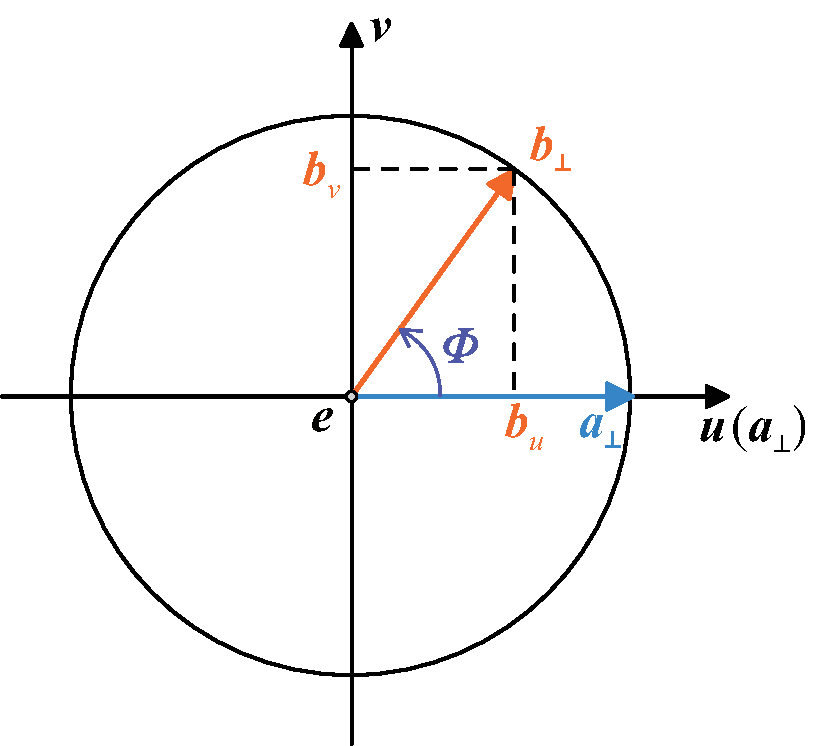
\includegraphics[width=\linewidth]{pic/欧拉轴2}
		\caption{欧拉轴旋转投影图}
		\label{欧拉轴2}
	\end{minipage}
	\begin{minipage}{0.33\linewidth}
		\centering
		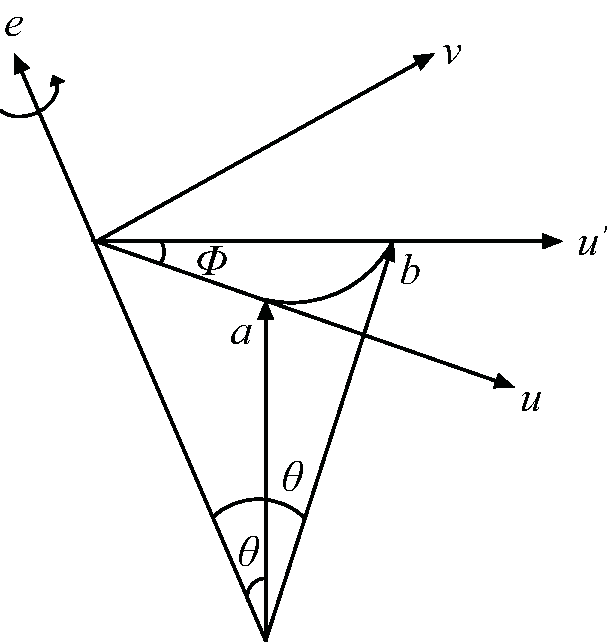
\includegraphics[width=0.913\linewidth]{pic/欧拉轴角}
		\caption{欧拉轴 / 角的坐标变换图}
		\label{欧拉轴角}
	\end{minipage}
\end{figure}

\noindent 将垂直分量$\bm{a}_{\perp}, \bm{b}_{\perp}$投影到垂直于轴$\bm{e}$的平面$\Pi$上,如图 \ref{欧拉轴2} 所示。定义单位正交矢量$\bm{u}, \bm{v}$
\begin{align*}
	\bm{u} & = \bm{a}_{\perp} = \dfrac{\bm{e} \times \bm{a}}{\big| \bm{e} \times \bm{a} \big|} = \dfrac{1}{a \sin \theta}(\bm{e} \times \bm{a}) \\
	\bm{v} & = \bm{e} \times \bm{u} = \dfrac{1}{a \sin \theta} \bm{e} \times (\bm{e} \times \bm{a})= \dfrac{1}{a \sin \theta}\big[ \bm{a} - (\bm{e} \cdot \bm{a})\bm{e} \big] 
\end{align*}
将矢量$\bm{b}_{\perp}$分解,得
\begin{equation*}
	\bm{b}_{\perp} = \cos \varPhi \bm{u} + \sin \varPhi \bm{v} = \cos \varPhi \bm{a}_\perp + \sin \varPhi (\bm{a}_\perp \times \bm{e})
\end{equation*}
将矢量$\bm{a}, \bm{b}$用上面的矢量表示为(注:$\bm{a}, \bm{b}$模长相等,即$a=b$)
\begin{align}
	\bm{a} & = a \big( \cos \theta \bm{a}_{\parallel} + \sin \theta \bm{a}_{\perp} \big) 
	= a \big( \cos \theta \bm{e} + \sin \theta \bm{v} \big) \\
	\bm{b} & = b \big( \cos \theta \bm{b}_{\parallel} + \sin \theta \bm{b}_{\perp} \big) 
	= a \big( \cos \theta \bm{e} + \sin \theta \bm{b}_{\perp} \big)
\end{align}
将$\bm{b}_{\perp}$的表达式反代,可以得到
\begin{equation}
	\bm{b} = \cos \varPhi \bm{a} + ( 1 - \cos \varPhi ) (\bm{e} \cdot \bm{a})\bm{e} + \sin \varPhi(\bm{e} \times \bm{a})
\end{equation}
分别取$\bm{a} = \bm{i}_a, \bm{j}_a, \bm{k}_a; \bm{b} = \bm{i}_b, \bm{j}_b, \bm{k}_b$,可以得到
\begin{equation}
	\begin{cases}
		\, \bm{i}_b = \cos \varPhi \bm{i}_a+ ( 1 - \cos \varPhi ) (\bm{e} \cdot \bm{i}_a)\bm{e} + \sin \varPhi(\bm{e} \times \bm{i}_a) \\
		\, \bm{j}_b = \cos \varPhi \bm{j}_a+ ( 1 - \cos \varPhi ) (\bm{e} \cdot \bm{j}_a)\bm{e} + \sin \varPhi(\bm{e} \times \bm{j}_a) \\
		\, \bm{k}_b = \cos \varPhi \bm{k}_a+ ( 1 - \cos \varPhi ) (\bm{e} \cdot \bm{k}_a)\bm{e} + \sin \varPhi(\bm{e} \times \bm{k}_a)
	\end{cases}
	\label{eq:zj}
\end{equation}
将$\bm{e}$在坐标系$S_a$中分解为$\bm{e} = e_x \bm{i}_a + e_y \bm{j}_a + e_z \bm{k}_a $,代入公式 \eqref{eq:zj} 合并即可。
\vspace*{0.8em}


\sssection[由方向余弦矩阵确定欧拉轴 / 角参数]

若已知方向余弦矩阵$\bm{C}_{ba}$,可以计算得到欧拉轴 / 角参数,得
\begin{align}
	\cos \varPhi = \dfrac{\text{tr} \bm{C}_{ba} - 1}{2} \\
	\bm{e} = \dfrac{1}{2 \sin \varPhi} 
	\begin{bmatrix}
		C_{23} - C_{32} \\
		C_{31} - C_{13} \\
		C_{12} - C_{21}
	\end{bmatrix}
\end{align}
其中,$\text{tr} \bm{C}_{ba}$是方向余弦矩阵的迹,$\text{tr} \bm{C}_{ba} = C_{11} + C_{12} + C_{13}$。绕任意轴转动相同的$\varPhi$角,方向余项矩阵的迹不变。
\clearpage

\noindent 将公式展开,对应得到以下3组解:

\noa[1] 当$\text{tr} \bm{C}_{ba} \neq 3, -1$时,可以直接计算分量$e_x, e_y, e_z$。

\noa[2] 当$\text{tr} \bm{C}_{ba} = 3$时,此时对应转角$\varPhi = 0, \pm 2 \pi, \pm 4 \pi, \cdots$,方向余弦矩阵$\bm{C}_{ba}$为单位矩阵,$e_x, e_y, e_z$无法确定。这种情况相当于没有发生转动。

\noa[3] 当$\text{tr} \bm{C}_{ba} = -1$时,对应转角$\varPhi = \pm \pi, \pm 3 \pi, \pm 5 \pi, \cdots$,此时$\bm{C}_{ba} = 2 \bm{e}\bm{e}^{\text{T}} - \bm{E}_3$,则有
\begin{equation}
	\begin{cases}
		\, e_x = \pm \sqrt{\dfrac{1 + C_{11}}{2}}, \qquad e_y = \pm \sqrt{\dfrac{1+ C_{22}}{2}}, \qquad e_z = \pm \sqrt{\dfrac{1 + C_{33}}{2}} \\[0.5em]
		\, e_x e_y = \dfrac{1}{2} C_{12}, \hspace*{3.7em} e_ye_z = \dfrac{1}{2}C_{23}, \hspace*{3.7em} e_ze_x = \dfrac{1}{2} C_{31}
	\end{cases}
\end{equation}
其中,使用后三个方程来判断前三个方程的符号。

\begin{figure}[!htb]
	\centering
	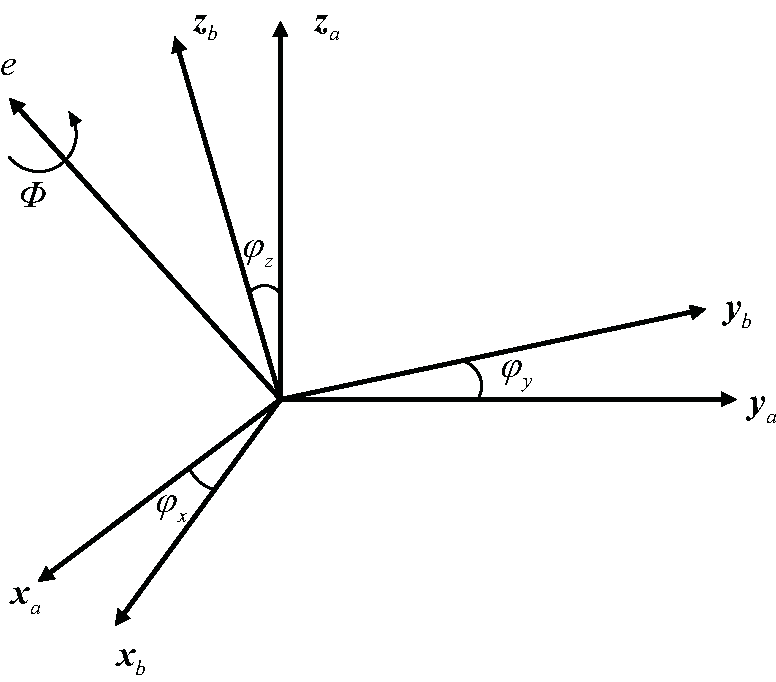
\includegraphics[width=0.4\linewidth]{pic/欧拉轴角变换}
	\vspace*{-1em}
	\caption{欧拉转角与两个坐标系之间的几何关系}
	\label{欧拉转角变换}
\end{figure}


\sssection[欧拉转角的几何意义]

如图 \ref{欧拉转角变换} 所示,令$\varphi_x, \varphi_y, \varphi_z$分别为两个坐标系对应轴之间的夹角,方向余弦矩阵的对焦线上的元素即为这几个角的余弦值,所以
\begin{equation}
	2 \cos \varPhi = \text{tr} \bm{C}_{ba} - 1 = \cos \varphi_x + \cos \varphi_y + \cos \varphi_z - 1
\end{equation}
利用半角公式$\cos \alpha = 1 - 2 \sin^2 \dfrac{\alpha}{2}$,则
\begin{equation}
	\sin^2 \dfrac{\varPhi}{2} = \dfrac{1}{2} \left( \sin^2 \dfrac{\varphi_x}{2} + \sin^2 \dfrac{\varphi_y}{2} + \sin^2 \dfrac{\varphi_z}{2} \right)
\end{equation}

当偏角较小时,有
\begin{equation}
	\varPhi \approx \dfrac{\sqrt{2}}{2} \sqrt{\varphi_x^2 + \varphi_y^2 + \varphi_z^2}
\end{equation}
这个公式对于评价旋转误差是很有用的。




\subsection{四元数}
\sssection[四元数的定义\footnote{四元数章节中的部分内容参考Github上Krasjet的讲义Quaternion\cite{Quaternion}}]

\defination[四元数]
{
	\dy[四元数]{SYS}的定义和复数类似,唯一的区别就是四元数一共有三个虚部,而复数只有一个。所有的四元数$q \in \mathbb{H}$($\mathbb{H}$代表四元数的发现者 William Rowan Hamilton)都可以写成下面这种形式
	\vspace*{-0.7em}
	\begin{equation}
		q = a + b i + cj +dk \quad (a,b,c,d \in \mathbb{R})
		\vspace*{-0.7em}
	\end{equation}
	其中,
	\vspace*{-0.7em}
	\begin{equation}
		i^2 = j^2 = k^2 = i j k = -1
	\end{equation}
}

四元数可以写成向量形式
\begin{equation}
	q = 
	\begin{bmatrix}
		a \\
		b \\
		c \\
		d
	\end{bmatrix}
\end{equation}
同时,通常将四元数的实部与虚部分开,并用一个三维的向量来表示虚部,将它表示为\dy[标量向量有序对]{BLXLYXD}形式
\begin{equation}
	q = \big[ s, \bm{v} \big],
	\quad 
	\bm{v} = 
	\begin{bmatrix}
		x \\
		y \\
		z
	\end{bmatrix} 
	\quad (s,x,y,z \in \mathbb{R})
\end{equation}


\sssection[四元数的模长]
\vspace*{-0.5em}

\defination[四元数的模长]
{
	\dy[四元数的模长]{SYSDMC}(范数)定义为
	\begin{equation}
		\norm[q] = \sqrt{a^2 + b^2 + c^2 + d^2}
	\end{equation}
	用标量向量有序对表示为
	\begin{equation}
		\norm[q] = \sqrt{s^2 + \norm[\bm{v}]^2} = \sqrt{s^2 + \bm{v} \cdot \bm{v}}
	\end{equation}
	\textbf{注:由于四元数是四维向量,其没有明确的物理几何意义。}
}
\vspace*{0.5em}


\sssection[四元数的加减运算]

四元数的加减运算和复数一致,设两个四元数为$q_1 = a + bi + cj + dk,\, q_2 = e + fi +gj + hk$,则
\begin{align}
	q_1 \pm q_2 & = a + bi + cj + dk \pm (e + fi +gj + hk) \notag \\
	& = (a \pm e)  + (b \pm f) i + (c \pm g) j + (d \pm h) k
\end{align}
标量向量对形式的加减与标量和向量的加减运算一致,设两个四元数为$q_1 = \big[s, \bm{v}\big],\, q_2 = \big[ t, \bm{u} \big]$,则
\begin{equation}
	q_1 \pm q_2 = \big[ s \pm t, \bm{v} \pm \bm{u} \big]
\end{equation}


\sssection[四元数的数乘]

一个四元数$q = a +bi +cj +dk$和标量$s$的乘积为
\begin{align}
	sq &= s (a + bi +cj +dk) \notag \\
	& = sa + sbi +scj +sdk
\end{align}
四元数的数乘运算满足交换律,即$sq = qs$.
\vspace*{1em}


\sssection[四元数的乘法]

四元数的乘法和矩阵乘法类似,不遵守交换律,即在一般情况下$q_1 q_2 \neq q_2 q_1$。所以,四元数乘法和矩阵乘法一样有左乘和右乘的区别。即

\noa[1] $q_1 q_2$\quad $q_1\,$\dy[左乘]{ZC}$\,q_2$\quad 或\quad $q_2\,$\dy[右乘]{YC}$\,q_1$.

\noa[2] $q_2 q_1$\quad $q_1\,$\dy[右乘]{YC}$\,q_2$\quad 或\quad $q_2\,$\dy[左乘]{ZC}$\,q_1$.

四元数的乘法满足结合律和分配律。
\clearpage

那么,如果有两个四元数$q_1 = \big[s, \bm{v}\big],\, q_2 = \big[ t, \bm{u} \big]$,则
\begin{align}
	q_1 q_2 & = (a + bi +cj +dk)(e + fi +gj +hk) \notag  \\
	& = ae + afi + agj + ak \notag \\
	& + bei + bfi^2 + bgij + bhik \notag \\
	& + cej + cfji + cgj^2 + chjk \notag \\
	& + dek + dfki + dgkj + dhk^2
\end{align}
利用四元数的性质$i^2 = j^2 = k^2 = i j k = -1$,可以得到
\begin{align}
	 ijk = -1 \, &\xrightarrow{\quad \textstyle \mbox{等式两边同时左乘} \,\, i \quad } \, iijk = -i \hspace*{-8em} &&\Rightarrow \quad jk = i \\
	 ijk = -1 \, &\xrightarrow{\quad \textstyle \mbox{等式两边同时右乘} \,\, k \quad } \, ijkk = -k \hspace*{-8em} &&\Rightarrow \quad ij = k \\
	 jk = i \, &\xrightarrow{\quad \textstyle \mbox{等式两边同时左乘} \,\, j \quad } \, jjk = ji  \hspace*{-8em} &&\Rightarrow \quad ji = -k \\
	 jk = i \, &\xrightarrow{\quad \textstyle \mbox{等式两边同时右乘} \,\, k \quad } \, jkk = ik  \hspace*{-8em} &&\Rightarrow \quad ik = -j \\
	 ij = k \, &\xrightarrow{\quad \textstyle \mbox{等式两边同时左乘} \,\, i \quad } \, iij = ik \hspace*{-8em} &&\Rightarrow \quad ik = -j \\
	 ij = k \, &\xrightarrow{\quad \textstyle \mbox{等式两边同时右乘} \,\, j \quad } \, ijj = kj \hspace*{-8em} &&\Rightarrow \quad kj = -i
\end{align}
将上面的性质整理为表格如表 \ref{四元数基本乘法} 所示。
\begin{table}[!htb]
	\centering
	\setlength{\tabcolsep}{2em}{
	\begin{tabular}{|c|c|c|c|c|}
		\hline
		\rowcolor{Azure2} $\times$ & 1 & $ i $ & $ j $ & $ k $ \\
		\hline
		\cellcolor{Azure2} 1 & 1 & $i$ & $j$ & $k$ \\
		\hline
		\cellcolor{Azure2} $i$ & $i$ & $-1$ &\cellcolor{MistyRose} $k$ & \cellcolor{DarkSlateGray2} $-j$ \\
		\hline
		\cellcolor{Azure2} $j$ & $j$ & \cellcolor{MistyRose} $-k$ & $-1$ & \cellcolor{LightGoldenrod1} $i$ \\
		\hline
		\cellcolor{Azure2} $k$ & $k$ & \cellcolor{DarkSlateGray2} $j$ &  \cellcolor{LightGoldenrod1} $-i$ & $-1$ \\
		\hline
	\end{tabular}
}
\caption{四元数基本向量的乘法计算表}
\label{四元数基本乘法}
\end{table}
\vspace*{-1em}

\summarize[
\hspace{1em} 记忆方法:类似于向量的叉乘,将$i,j,k$理解为三维右手坐标系,则$i \times j =k , j \times i = -k$,其余类似。
]

利用这个表格,可以将四元数乘法的结果化简为
\begin{align}
	q_1 q_2 & = ae + afi + agj + ak \notag \\
& + bei + bfi^2 + bgij + bhik \notag \\
& + cej + cfji + cgj^2 + chjk \notag \\
& + dek + dfki + dgkj + dhk^2 \notag \\
& = (a {\color{VioletRed} e} - b {\color{cyan} f} - c{\color{SeaGreen} g} - d{\color{orange} h}) \notag \\
& + (b {\color{VioletRed} e} - a {\color{cyan} f} - d{\color{SeaGreen} g} - c{\color{orange} h}) i \notag \\
& + (c {\color{VioletRed} e} - d {\color{cyan} f} - a{\color{SeaGreen} g} - b{\color{orange} h}) j \notag \\
& + (d {\color{VioletRed} e} - c {\color{cyan} f} - b{\color{SeaGreen} g} - a{\color{orange} h}) k
\end{align}
写成矩阵为
\begin{equation}
		q_1 q_2 = 
		\begin{bmatrix}
			a & -b & -c & -d \\
			b & a & -d & c \\
			c & d & a & -b \\
			d & -c & b & a
		\end{bmatrix}
		\,\, 
		\begin{bmatrix}
		 {\color{VioletRed} e} \\
		 {\color{cyan} f} \\
		 {\color{SeaGreen} g} \\
		 {\color{orange} h} 
		\end{bmatrix}
\end{equation}
同理可得,右乘的结果为
\begin{equation}
	q_2 q_1 = 
	\begin{bmatrix}
		a & -b & -c & -d \\
		b & a & d & c \\
		c & -d & a & b \\
		d & c & -b & a
	\end{bmatrix}
	\,\, 
	\begin{bmatrix}
		{\color{VioletRed} e} \\
		{\color{cyan} f} \\
		{\color{SeaGreen} g} \\
		{\color{orange} h} 
	\end{bmatrix}
\end{equation}
\vspace*{0.5em}


\sssection[Grassmann 积]

为了将四元数的结果写成标量向量有序对,重新整理结果
\begin{align}
	q_1 q_2 & = (ae - ({\color{SeaGreen}bf + cg + dh})) \notag \\
	& + (b {\color{VioletRed} e} + {\color{cyan} a}f +{\color{orange} ch - dg} ) i \notag \\
	& + (c {\color{VioletRed} e} + {\color{cyan} a}g +{\color{orange} df - bh} ) j \notag \\
	& + (d {\color{VioletRed} e} + {\color{cyan} a}h +{\color{orange} bg - cf} ) k \notag 
\end{align}
令
$
\bm{v} = 
\begin{bmatrix}
	b \\
	c \\
	d
\end{bmatrix}
, \,
\bm{u} = 
\begin{bmatrix}
	f \\
	g \\
	h
\end{bmatrix}
$,那么
\begin{align*}
	\bm{v} \cdot \bm{u} &= {\color{SeaGreen}bf + cg + dh} \\
	\bm{v} \times \bm{u} &= 
	\begin{vmatrix}
		\bm{i} & \bm{j} & \bm{k} \\
		b & c & d \\
		f& g & h
	\end{vmatrix}
= ({\color{orange} ch - dg}) \bm{i} + ({\color{orange} df - bh} )\bm{j} + ({\color{orange} bg - cf} )\bm{k}
\end{align*}
所以,$q_1q_2$的结果可以用向量点乘和叉乘的形式表示出来\footnote{其实按照历史的顺序来说,这里第一次提出叉乘的概念。}
\begin{equation}
	q_1 q_2 = \big[ ae - \bm{v} \cdot \bm{u}, a\bm{u} +e \bm{v} + \bm{v} \times \bm{u} \big]
\end{equation}

这个结果称为\dy[Grassmann积]{GRASSMANNJ},一般来说

\theorem[Grassmann 积]
{
	对于任意四元数$q_1= \big[s, \bm{v} \big],\, q_2= \big[ t, \bm{u} \big]$,$q_1q_2$的结果为
	\begin{equation}
		q_1 q_2 = \big[ st - \bm{v} \cdot \bm{u}, s \bm{u} + t \bm{v} + \bm{v} \times \bm{u} \big]
	\end{equation}
}
\vspace*{0.5em}


\sssection[四元数的逆]

因为四元数不遵守交换律,所以类似于矩阵除法,四元数相除等价于乘以它的逆。同样地,也有左除和右除之分,即$pq^{-1}$或$q^{-1}p$,它们的结果一般不同。

\clearpage

\vspace*{-2em}
\defination[四元数的逆]
{
	如果
	\begin{equation}
		qq^{-1} = q^{-1} q = 1 \quad (q \neq 0)
	\end{equation}
	那么,我们称$q^{-1}$为四元数$q$的\dy[逆]{N}。
}

直接求解一个四元数的逆$q^{-1}$是非常困难的,但是我们可以使用四元数共轭的性质来求$q^{-1}$。
\vspace*{1em}


\sssection[共轭四元数]
\vspace*{-0.5em}

\defination[共轭四元数]
{
	一个四元数$q = a + bi + cj + dk$的\dy[共轭]{GE}为
	\begin{equation}
		q^* = a - bi - ci -dk
	\end{equation}
	如果用标量向量有序对的形式来定义,则$q = \big[ s, \bm{v} \big]$的\dy[共轭]{GE}为
	\begin{equation}
		q^* = \big[ s, -\bm{v} \big]
	\end{equation}
}

共轭四元数的一个非常有用的性质就是
\begin{align}
	q q^* &= \big[s, \bm{v}] \cdot \big[s, - \bm{v}] \notag \\
	& = \big [s^2 - \bm{v} \cdot \bm{v}, s(- \bm{v}) + s \bm{v} + \bm{v} \times (- \bm{v})] \notag \\
	& = \big[s^2 + \bm{v}\cdot \bm{v}, 0] \notag \\
	& = s^2 + x^2 + y^2 + z^2 = \norm[q]^2 \quad \left(\bm{v} = \big[ x, y, z \big]^{\text{T}}\right) 
\end{align}
因为$(q^*)^* = \big [s, - (- \bm{v})] = \big[s, \bm{v}\big] = q$,则
\begin{equation}
	q^* q = (q^*)(q^*)^* = \norm[q^*]^2 = s^2 + x^2 +y^2 + z^2 = \norm[q]^2 = q q^* 
\end{equation}
这说明,$q^*q = qq^*$。这个特殊的乘法是遵守交换律的。

下面利用四元数的性质求四元数的逆。
\begin{align*}
	q q^{-1} = 1 \, \xrightarrow{\textstyle \quad \mbox{等式两边同时左乘}\, q^* \quad }\, q^* q q^{-1} = 1 &\quad \Rightarrow \quad (q^* q)q^{-1} = q^* \, \xrightarrow{\quad \textstyle q^* q = \norm[q]^2 \quad } \norm[q]^2 \cdot q^{-1} = q^* \notag
\end{align*}
由此可知

\theorem[四元数逆的求解]
{
	四元数的逆可以表示为
	\begin{equation}
		q^{-1} = \dfrac{q^*}{\norm[q]^2}
	\end{equation}
	用这种方法寻找一个四元数的逆会非常高效,我们只需要将一个四元数的共轭除以它的模长的平方就可以得到四元数的逆。特别地对于\dy[单位四元数]{DWSYS}$\norm[q] = 1$来说,它的逆为
	\begin{equation}
		q^{-1} = \dfrac{q^*}{1^2} = q^*
	\end{equation}
}

\clearpage

\sssection[纯四元数]
\vspace*{-0.5em}

\defination[纯四元数]
{
	如果一个四元数实部为0,仅有虚部,即
	\begin{equation}
		v = \big[ 0, \bm{v} \big]
	\end{equation}
	那么我们则称这个四元数$v$为一个\dy[纯四元数]{CXYS}。因为纯四元数仅由虚部的3D向量决定,我们可以将任意的3D向量转换为纯四元数。
}

纯四元数有一个很重要的特性:两个纯四元数$v = \big[ 0, \bm{v} \big], u = \big[ 0, \bm{u} \big]$的乘积为
\begin{align}
	vu &= \big[ 0 - \bm{v} \cdot \bm{u}, 0 + \bm{v} \times \bm{u} \big] \notag \\
	& = \big[ - \bm{v} \cdot \bm{u}, \bm{v} \times \bm{u} \big]
	\label{eq: 纯四元数乘法}
\end{align}
\vspace*{0.5em}




\sssection[四元数与3D旋转]

\begin{figure}[!htb]
	\centering
	\begin{minipage}{0.31\linewidth}
		\centering
		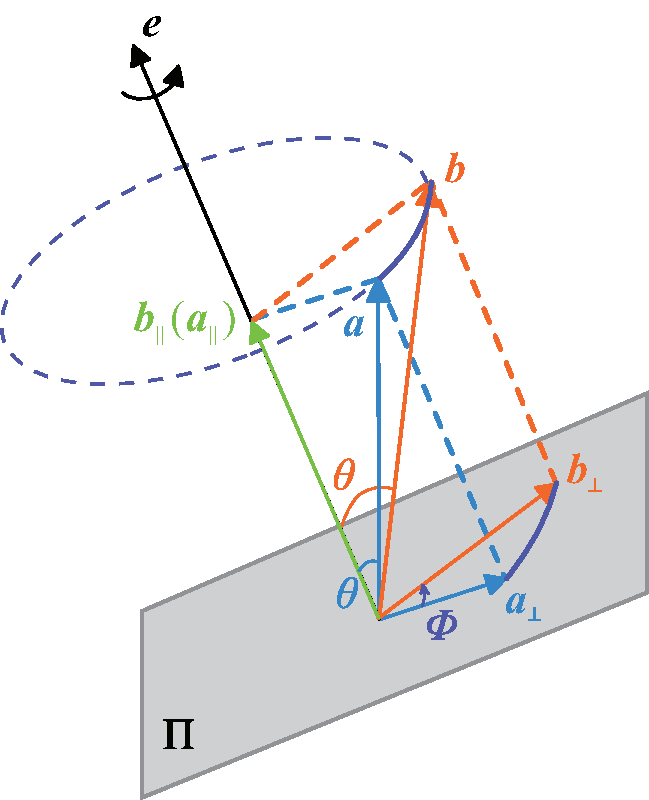
\includegraphics[width=0.9\linewidth]{pic/欧拉轴}
		\vspace*{-1.2em}
		\caption{向量旋转分解图}
		\label{欧拉轴3}
	\end{minipage}\hspace*{7em}
	\begin{minipage}{0.348\linewidth}
		\centering
		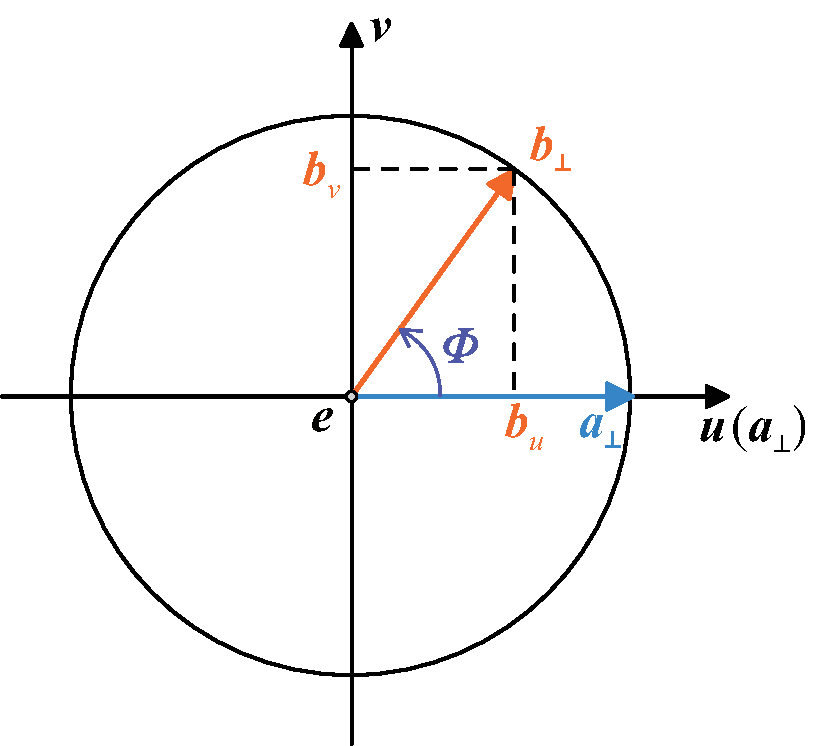
\includegraphics[width=\linewidth]{pic/欧拉轴2}
		\caption{向量旋转投影图}
		\label{欧拉轴4}
	\end{minipage}
\end{figure}

在上个章节 \ref{sec: 欧拉轴角} 中我们知道:如果我们需要将一个向量$\bm{a}$沿着一个用单位向量$\bm{e}$所定义的旋转轴旋转$\varPhi$度,那么我们可以将这个向量$\bm{a}$可以分解为平行于旋转轴的分量$a_{\parallel}$和垂直于旋转轴的分量$a_{\perp}$。旋转后得到的向量$\bm{b}$可以表示为这两个分量分别旋转后之和,即$\bm{b} = \bm{b}_{\parallel} + \bm{b}_{perp}$。

我们定义这些向量为纯四元数
\begin{align*}
	a &= \big[ 0, \bm{a} \big]  && b = \big[ 0, \bm{b} \big] \\
	a_\perp &= \big[ 0, \bm{a}_\perp \big] && b_\perp = \big[ 0, \bm{b}_\perp \big] \\
	a_\parallel &= \big[ 0, \bm{a}_\parallel \big] && b_\parallel = \big[ 0, \bm{b}_\parallel \big] \\
	e &= \big[0, \bm{e} \big] 
\end{align*}
那么我们可以得到
\begin{equation*}
	a = a_\parallel + a_\perp \qquad \qquad b = b_\parallel + b_\perp
\end{equation*}

如图 \ref{欧拉轴3} 所示,我们知道,旋转前后平行分量$\bm{a}_{\parallel} = \bm{b}_{\parallel} = \bm{e}$相等,即旋转前后不变,下面考虑垂直分量$\bm{a}_{\perp}$的旋转。

在上个章节 \ref{sec: 欧拉轴角} 中我们推导过垂直分量$\bm{a}_{\perp}$的旋转公式
\begin{equation*}
	\bm{b}_{\perp} = \cos \varPhi \bm{a}_\perp + \sin \varPhi (\bm{e} \times \bm{a}_\perp )
\end{equation*}

我们可以很容易将$a'_\perp$和$a_\perp$写成四元数的形式,而对于$\bm{a}_\perp \times \bm{e}$,由纯四元数的重要性质,由\eqrefp[eq: 纯四元数乘法]可知,纯四元数$a = \big[ 0, \bm{a_\perp}\big], \, e = \big[ 0, \bm{e} \big]$,那么
\begin{equation*}
	ea_\perp = \big[ - \bm{e} \cdot \bm{a}_\perp, \bm{e} \times \bm{a}_\perp \big]
\end{equation*}
而$\bm{e} \perp \bm{a}_\perp \,\, \Rightarrow \,\, \bm{e} \cdot \bm{a}_\perp = 0$,所以
\begin{align*}
	ea_\perp & = \big[ 0, \bm{e} \times \bm{a}_\perp \big] \\
	& = \bm{e} \times \bm{a}_\perp
\end{align*}
所以$\bm{a}_{\perp}$旋转公式的四元数表达为
\begin{align}
	b_\perp &= \cos \varPhi a_\perp + \sin \varPhi (ea_\perp)\\
	& = \big( \cos \varPhi + \sin \varPhi e \big) a_\perp 
\end{align}

令$q = \cos \varPhi + \sin \varPhi e$,则可以得到
\begin{equation}
	b_\perp = q a_\perp
\end{equation}
所以,我们只需要构造一个四元数$q$,就可以完成垂直分量的旋转。对$q$进一步变形,得
\begin{align}
	q &= \cos \varPhi + \sin \varPhi u \notag \\
	& = \big[ \cos \varPhi, \bm{0} \big] + \big[ 0, \sin \varPhi \bm{e} \big] \notag \\
	& = \big[ \cos \varPhi , \sin \varPhi \bm{e} \big] 
\end{align}

如果已经知道旋转轴的坐标
$
\bm{e} = 
\begin{bmatrix}
	e_x \\
	e_y \\
	e_z
\end{bmatrix}
$
和旋转角$\varPhi$,那么四元数$q$就确定为
\begin{equation}
	q = \big[ \cos \varPhi , \sin \varPhi \bm{e} \big]  = \cos \varPhi + \sin \varPhi e_x i + \sin \varPhi e_y j + \sin \varPhi e_z k
\end{equation}
四元数$q$还有一个性质(注:$\norm[\bm{u}] = 1$)
\begin{align}
	\norm[q] &= \sqrt{\cos^2 \varPhi + (\sin\varPhi \bm{u} \cdot \sin \varPhi \bm{u})} \notag \\
	& = \sqrt{\cos^2 \varPhi + \sin^2 \varPhi(\bm{u} \cdot \bm{u})} \notag \\
	& = \sqrt{\cos^2 \varPhi+ \sin^2 \varPhi} = 1
\end{align}
说明旋转四元数参数$q$是单位四元数,一定意义上表面它所做的变换并不会对原向量进行缩放,是一个纯旋转。
\vspace*{1em}

又因为平行分量旋转前后不改变,即$\bm{b}_\parallel = \bm{a}_\parallel \,\, \Rightarrow \,\,  b_ \parallel = a_ \parallel $所以,向量$\bm{a}$的最终四元数旋转表示为
\begin{align}
	b &= b_\parallel + b_\perp \notag \\
	&= a_\parallel + q a_\perp \qquad \mbox{(其中}\,\, q = \big[ \cos \varPhi, \sin \varPhi \bm{e}\big]\mbox{)}
\end{align}
通过进一步的化简\footnote[1]{由于篇幅所限,此部分化简内容请参见 第 \ref{参考内容} 章 \link[参考内容]: \ref{旋转四元数参数的化简} \link[旋转四元数参数的化简]},可以得到

\clearpage 

\vspace*{-2em}
\theorem[旋转四元数参数]
{
	任意向量$\bm{a}$沿着以单位向量定义的旋转轴$\bm{e}$旋转$\varPhi$度之后的向量$\bm{b}$可以用四元数表达。令$a = \big[ 0, \bm{a} \big], \, q = \left[ \cos \left(\dfrac{1}{2} \varPhi \right), \sin \left(\dfrac{1}{2} \varPhi \right) \bm{a} \right]$,那么
	\begin{equation}
		b = q a q^* = q a q^{-1}
	\end{equation}
	为了更好的理解这个公式的意义,我们可以得到\footnotemark[1]
	\begin{equation}
		b = q a q^* = q q^* a_\parallel + qqa_\perp = a_\parallel + q^2 a_\perp
		\label{旋转四元数的几何意义}
	\end{equation}
	也就是说,$qaq^*$这个变换,实际上可以等价为,对$a$平行于坐标轴的分量$a_\parallel$实施的变换是$qq^*$,这两个变换是互逆的,完全抵消了,也就是没有旋转。而对于正交于旋转轴的分量$a_\perp$,则实施的是两次完全一样的变换$q^2 = qq$,将它旋转$\dfrac{\varPhi}{2} + \dfrac{\varPhi}{2} = \varPhi$度。
}

\footnotetext[1]{公式 \eqref{旋转四元数的几何意义} 是原式公式化简第一步的结果,详情请见\eqrefp[旋转几何意义]。}







